\documentclass[10pt]{ctexart}
\usepackage{ylsart}
\usepackage{enumerate}
\usepackage{bm}
\usepackage{makecell}
\usepackage{xcolor}
\usepackage{graphicx}
\usepackage{subfigure}
\usepackage{framed}%包中有添加文字背景色命令shaded
\colorlet{shadecolor}{MaterialBlue50}
\usepackage{tabularx}
\usepackage{multicol}  
\usepackage{multirow}
\usepackage{indentfirst}
\usepackage{amsmath,amssymb,amsthm,bm,bbding,pifont,dsfont}
\usepackage{mathtools}
\newcommand{\abs}[1]{\left| #1 \right|}
\usepackage{caption}
\captionsetup[figure]{labelfont={bf},labelformat={default},labelsep=period,name={图}}
%定义选择题选项
\newcommand{\onech}[4]{
\renewcommand\arraystretch{1.4}
\begin{tabularx}{\linewidth}{XXXX}
\setlength\tabcolsep{0pt}
(A) #1 & (B) #2 & (C) #3 & (D) #4 \\
\end{tabularx}
\unskip \unskip}
\newcommand{\twoch}[4]{
\renewcommand\arraystretch{1.4}
\begin{tabularx}{\linewidth}{XX}
\setlength\tabcolsep{0pt}
(A) #1 & (B) #2 \\
(C) #3 & (D) #4
\end{tabularx}
\unskip \unskip}

\newcommand{\jd}[1]{\noindent {\kaishu \textbf{解:}#1}}
\newcommand\pxx{%
		\mathrel{\text{\tikz[baseline] \draw (0em,-0.3ex) -- (.4em,1.7ex) (.2em,-0.3ex) -- (.6em,1.7ex);}%
	}}



\title{\huge\heiti 三角形面积公式全归纳}
\author{初中数学中有关三角形面积计算应该掌握的公式\\一粒沙}
\date{\today}



\begin{document}
\maketitle
\tableofcontents


\section{引入}
同一平面内,不在同一直线的三条线段首尾顺次相接所组成的封闭图形叫做三角形,符号为$\triangle$。求三角形面积对于初中学生来说似乎很简单,毕竟好像每位同学都知道三角形面积公式;但是往往中考有可能就针对同学们的得意之处入手,改变游戏规则,使得正常的三角形面积公式无法适用,因为问题中不会直接告诉我们三角形的底和高,最常见的是在反比例函数和二次函数中,因此掌握一些必要的公式是很有用的。
\section{三角形面积公式全归纳}

\begin{minipage}[t]{0.7\textwidth}
\begin{dkli}{}{}
已知三角形的底边长为$a$,底边上的高为$h$,则三角形的面积:
\[S=\text{底}\times \text{高}\div 2=\dfrac{1}{2}ah\]
\end{dkli}
\end{minipage}
\begin{minipage}[t]{0.3\textwidth}
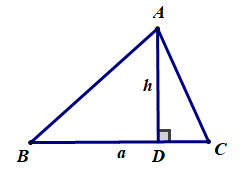
\includegraphics[scale=0.6]{figure/mj-01.png}
\end{minipage}

\begin{minipage}[t]{0.7\textwidth}
\begin{dkli}{}{}
已知三角形的两边及其夹角,则三角形的面积:
\[S=\dfrac{1}{2}ab \sin{C}=\dfrac{1}{2}bc \sin{A}=\dfrac{1}{2}ac \sin{B}\]
该公式是高中学习正余弦定理后学习的,但如果能让初中学生记住该公式可以对相关习题秒杀。
\end{dkli}
\end{minipage}
\begin{minipage}[t]{0.3\textwidth}
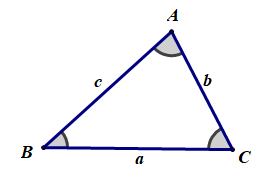
\includegraphics[scale=0.6]{figure/mj-02.png}
\end{minipage}

\begin{minipage}[t]{0.7\textwidth}
\begin{dkli}{}{}
海伦-秦九韶公式:已知$\triangle ABC$中,$AB=c,AC=b,BC=a$,
$p=\dfrac{1}{2}(a+b+c)$,称为三角形的半周长,则三角形的面积:
\[S=\sqrt{p(p-a)(p-b)(p-c)}\]
该公式实际是由中国古代著名数学家秦九韶首先发现的,在初中数学教材中二次根式内容章节后有介绍,记住该公式对初中学生求三角形面积有很大帮助。
\end{dkli}
\end{minipage}
\begin{minipage}[t]{0.3\textwidth}
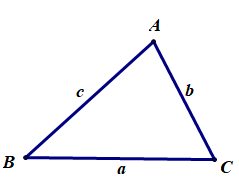
\includegraphics[scale=0.6]{figure/mj-03.png}
\end{minipage}

\begin{minipage}[t]{0.7\textwidth}
\begin{dkli}{}{}
在平面直角坐标系中,$\triangle ABC$的三个顶点坐标分别为$A(x_1,y_1),\\B(x_2,y_2),C(x_3,y_3)$,则三角形的面积:
\[S=\dfrac{1}{2}\left|x_1y_2+x_2y_3+x_3y_1-x_1y_3-x_2y_1-x_3y_2\right|\]
对于初中学生可以这样处理:先算出任意两组点的坐标差值,再代入下面公式计算即可,例如计算$A,B$和$A,C$的坐标差值:
\[AB=(x_2-x_1,y_2-y_1),AC=(x_3-x_1,y_3-y_1)\]
然后计算三角形面积为:
\[S=\dfrac{1}{2}\left|(x_2-x_1)(y_3-y_1)-(x_3-x_1)(y_2-y_1)\right|\]即$AB$和$AC$的坐标差值交叉相乘相减。

在初中数学里平面直角坐标系内容章节中经常出现已知三角形三顶点坐标求面积的问题(有时可能是四边形等,但可以转化为三角形),该公式对这类问题秒杀。
\end{dkli}
\end{minipage}
\begin{minipage}[b]{0.3\textwidth}
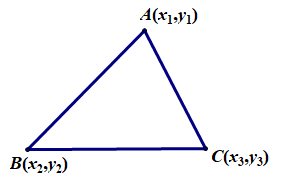
\includegraphics[scale=0.6]{figure/mj-04.png}\\
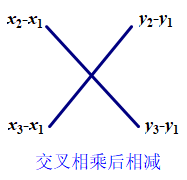
\includegraphics[scale=0.6]{figure/mj-shizi.png}
\end{minipage}

\begin{minipage}[t]{0.7\textwidth}
\begin{dkli}{}{}
已知三角形的三边长为$a,b,c$或周长,内切圆的半径为$r$,则三角形的面积:
\[S=pr=\dfrac{1}{2}(a+b+c)r,p=\dfrac{1}{2}(a+b+c)\]
\end{dkli}
\end{minipage}
\begin{minipage}[t]{0.3\textwidth}
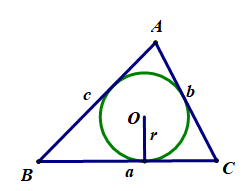
\includegraphics[scale=0.6]{figure/mj-05.png}
\end{minipage}

\begin{minipage}[t]{0.7\textwidth}
\begin{dkli}{}{}
已知三角形的三边长为$a,b,c$或三边积为$l=abc$,外接圆的半径为$R$,则三角形的面积:
\[S=\dfrac{abc}{4R}=\dfrac{l}{4R}\]
\end{dkli}
\end{minipage}
\begin{minipage}[t]{0.3\textwidth}
\qquad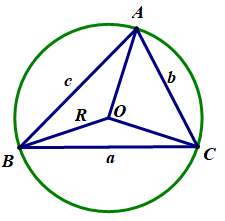
\includegraphics[scale=0.5]{figure/mj-06.png}
\end{minipage}

\begin{minipage}[t]{0.7\textwidth}
\begin{dkli}{}{}
已知三角形的三个顶点$A,B,C$到内切圆的切线长分别为$x,y,z$,如右图所示,则三角形的面积:
\[S=\sqrt{xyz(x+y+z)}\]
\end{dkli}
\end{minipage}
\begin{minipage}[t]{0.3\textwidth}
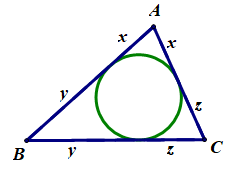
\includegraphics[scale=0.6]{figure/mj-07.png}
\end{minipage}

\begin{minipage}[t]{0.7\textwidth}
\begin{dkli}{}{}
已知三角形两角及其夹边,则三角形面积公式为:
\[S=\dfrac{a^2 \sin{B} \sin{C}}{2\sin(B+C)}=\dfrac{b^2 \sin{A} \sin{C}}{2\sin(A+C)}=\dfrac{c^2 \sin{A} \sin{B}}{2\sin(A+B)}\]
该公式利用诱导公式可以继续化简为:
\[S=\dfrac{a^2 \sin{B} \sin{C}}{2\sin A}=\dfrac{b^2 \sin{A} \sin{C}}{2\sin B}=\dfrac{c^2 \sin{A} \sin{B}}{2\sin C}\]
\end{dkli}
\end{minipage}
\begin{minipage}[t]{0.3\textwidth}
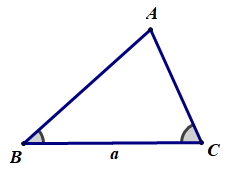
\includegraphics[scale=0.6]{figure/mj-08.png}
\end{minipage}


\begin{minipage}[t]{0.7\textwidth}
\begin{dkli}{}{}
已知三角形$ABC$的三条中线长为$u,v,w$,可利用下面公式求面积:
\[S=\dfrac{4}{3}\sqrt{s(s-u)(s-v)(s-w)}\]
其中$s=\dfrac{1}{2}(u+v+w)$.
\end{dkli}
\end{minipage}
\begin{minipage}[t]{0.3\textwidth}
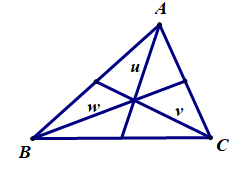
\includegraphics[scale=0.6]{figure/mj-11.png}
\end{minipage}

\begin{minipage}[t]{0.7\textwidth}
\begin{dkli}{}{}
如图,在三角形$ABC$中,水平宽为$l$,铅垂高为$k$,则三角形的面积为:
\[S=\dfrac{1}{2}lk\]
即三角形的面积等于水平宽与铅垂高乘积的一半。这种求面积的方法叫做铅垂法。在二次函数中,经常会求解三角形面积的最大值,我们常常需要使用这种方法。
\end{dkli}
\end{minipage}
\begin{minipage}[t]{0.3\textwidth}
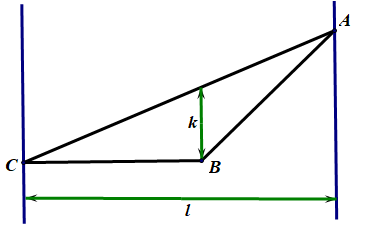
\includegraphics[scale=0.45]{figure/mj-12.png}
\end{minipage}

\begin{minipage}[t]{0.7\textwidth}
\begin{dkli}{}{}
已知三角形两角$B,C$及其对边$b,c$,则三角形面积公式为:
\[S=\dfrac{1}{2}c^2 \sin B \cos B+\dfrac{1}{2}b^2 \sin C \cos C\]
进一步化简即得下面公式:
\[S=\dfrac{1}{4}(c^2 \sin{2B}+b^2 \sin{2C})\]
\end{dkli}
\end{minipage}
\begin{minipage}[t]{0.3\textwidth}
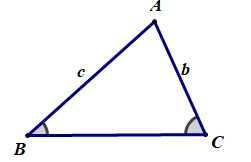
\includegraphics[scale=0.6]{figure/mj-09.png}
\end{minipage}

\begin{minipage}[t]{0.7\textwidth}
\begin{dkli}{}{}
由正弦定理结合上面公式可推出下面几组面积公式(其中$R$为三角形外接圆的半径,$r$为三角形内切圆的半径):
\begin{align*}
S&=2R^2 \sin A\sin B\sin C\\
S&=Rr(\sin A+\sin B+\sin C)\\
S&=4Rr \cos{\dfrac{A}{2}}\cos{\dfrac{B}{2}}\cos{\dfrac{C}{2}}\\
S&=\dfrac{1}{4}(a^2+b^2-c^2)\tan C(C\neq 0)
\end{align*}
\end{dkli}
\end{minipage}
\begin{minipage}[t]{0.3\textwidth}
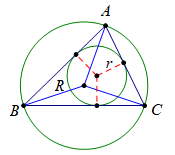
\includegraphics[scale=1]{figure/mj-17.png}
\end{minipage}


\begin{minipage}[t]{0.7\textwidth}
\begin{dkli}{}{}
已知三角形$ABC$的三边$a,b,c$和任意一内角,可利用下面公式求面积:
\[S=p(p-a)\tan{\dfrac{A}{2}}=p(p-b)\tan{\dfrac{B}{2}}=p(p-c)\tan{\dfrac{C}{2}}\]
其中$p=\dfrac{1}{2}(a+b+c)$
\end{dkli}
\end{minipage}
\begin{minipage}[t]{0.3\textwidth}

\end{minipage}

\begin{minipage}[t]{0.7\textwidth}
\begin{dkli}{}{}
由公式5和公式6可得出$Rr=\dfrac{abc}{2(a+b+c)}$,结合公式12可推出下面面积公式:
\[S=\dfrac{abc}{2(a+b+c)}(\sin{A}+\sin{B}+\sin{C})\]
\end{dkli}
\end{minipage}
\begin{minipage}[t]{0.3\textwidth}

\end{minipage}

\section[实例演练]{实例演练\footnote{例题中面积的求解方法可能有多种,本文仅说明利用上述公式来求解。}}

\begin{shaded}
\begin{example}
三边长分别为$13,14,15$的三角形,其面积是多少?内切圆和外接圆的半径是多少?
\end{example}
\end{shaded}
\jd 根据公式3,先计算$p=\dfrac{1}{2}(a+b+c)=21$,则面积为:$S=\sqrt{21(21-13)(21-14)(21-15)}=84$.\\
根据公式5,$84=21r,r=4$.\\
根据公式6,$R=\dfrac{abc}{4S}=\dfrac{13\times 14\times 15}{4\times 84}=\dfrac{65}{8}$.

\begin{shaded}
\begin{example}
三角形三边中线长分别为$3,4,5$,其面积是多少?
\end{example}
\end{shaded}
\jd 根据公式9,$s=\dfrac{1}{2}(3+4+5)=6,S=\dfrac{4}{3}\sqrt{6(6-3)(6-4)(6-5)}=8$.

\begin{shaded}
\begin{example}
在平面直角坐标系中,$\triangle ABC$的顶点坐标分别为$A(1,-1),B(-1,4),C(-3,1)$.

(1)求三角形$ABC$的面积;

(2)将$\triangle ABC$先向下平移2个单位,再向右平移3个单位,求线段$AB$扫过的面积。
\end{example}
\end{shaded}
\jd ~(1)根据公式4,$S=\dfrac{1}{2}\left|4-1+3-1+4+12\right|=21$.

    (2)略.


\begin{shaded}
\begin{example}
已知:$m,n$是方程$x^2-6x+5=0$的两个实数根,且$m<n$,抛物线$y=-x^2+bx+c$的图像经过点$A(-m,0),B(0,n)$.

$(1)$求这个抛物线的解析式;

$(2)$设(1)中抛物线与$x$轴的另一交点为$C$,抛物线的顶点为$D$,试求出点$C,D$的坐标和$\triangle BCD$的面积.
\end{example}
\end{shaded}
{\kaishu \textcolor{blue} {分析:求三角形$BCD$的面积,可以利用铅垂法,如图1过点$D$作$DE \pxx y$轴,交$BC$于点$E$,则铅垂高为$DE$,水平宽为$OC$。$DE$的长度=点$D$的坐标$-$点$E$的坐标;$OC$的长度=点$C$的坐标$-$点$O$的坐标.}}
\begin{minipage}[t]{0.6\textwidth}
\vspace{-4cm}
\jd (1)解方程$x^2-6x+5=0$得$m=1,n=5$,

则$A(-1,0),B(0,5)$,把$A(-1,0),B(0,5)$代入$y=-x^2+bx+c$,

得$\begin{cases}
-1-b+c=0 \\
c=5 \\
\end{cases}$,解得$\begin{cases}
b=4 \\
c=5 \\
\end{cases}$,

所以抛物线解析式为$y=-x^2+4x+5$;

(2)$y=-x^2+4x+5=-(x-2)^2+9$,则$D(2,9)$,

解方程$-x^2+4x+5=0$得$x_1=-1,x_2=5$,则$C(5,0)$.

设直线$BC$的解析式为$y=px+q$,

把$C(5,0),B(0,5)$代入得$\begin{cases}
5p+q=0 \\
q=5 \\
\end{cases}$,解得$\begin{cases}
p=-1 \\
q=5 \\
\end{cases}$,

$\therefore$直线$BC$的解析式为$y=-x+5$,

作$DE \pxx y$轴交$BC$于$E$,如图1,

则$E$点坐标为$(2,3)$,

$\therefore S_{\triangle BCD}=S_{\triangle BDE}+S_{\triangle CDE}=\dfrac{1}{2}\times (9-3)\times 5=15$.

\end{minipage}
\begin{minipage}[c]{0.4\textwidth}
  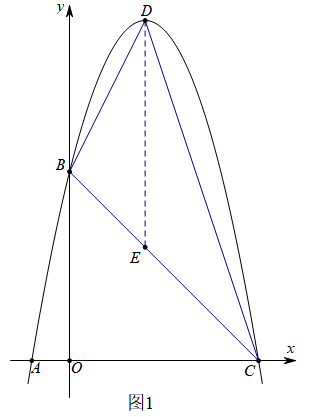
\includegraphics[scale=0.8]{figure/mj-16.png}
\end{minipage}

\begin{shaded}
\begin{example}
如图2,抛物线经过$A(4,0),B(1,0),C(0,-2)$三点.

(1)求这个抛物线的解析式;

(2)在直线$AC$上方抛物线上有一动点$D$,求使$\triangle DCA$的面积最大的点$D$的坐标.
\end{example}
\end{shaded}
{\kaishu \textcolor{blue} {分析:作$DE \pxx y$轴交$AC$于点$E$,如何求铅垂高$DE$?\textcolor{red}{利用设点法},先表示出点$D$和点$E$的坐标,点$D$与点$E$的横坐标是一样的,点$D$在抛物线上,点$E$在直线上,将横坐标代入解析式,就可求出纵坐标。设点$D(t,-\dfrac{1}{2}t^2+\dfrac{5}{2}t-2)$,则点$E(t,\dfrac{1}{2}t-2)$,铅垂高$DE$的长度=点$D$的纵坐标$-$点$E$的纵坐标,水平宽$OA$的长度=点$A$的横坐标$-$点$O$的横坐标。}}

\begin{minipage}[t]{0.6\textwidth}
\vspace{-5cm}
\jd (1)$\because$该抛物线过点$C(0,-2)$,

$\therefore$ 可设抛物线的解析式为$y=ax^2+bx-2$.

将$A(4,0),B(1,0)$代入,

得$\begin{cases}
16a+4b-2=0 \\
a+b-2=0 \\
\end{cases}$,解得$\begin{cases}
a=-\dfrac{1}{2}\\
b=\dfrac{5}{2}\\
\end{cases}$,\\[5pt]

故该二次函数的解析式为$y=-\dfrac{1}{2}x^2+\dfrac{5}{2}x-2$。\\[2pt]

(2)如图3,设点$D$的横坐标为$t(0<t<4)$,

则点$D$的纵坐标为$-\dfrac{1}{2}t^2+\dfrac{5}{2}t-2$.

由题意可求得直线$AC$的解析式为$y=\dfrac{1}{2}x-2$.

$\therefore E$点的坐标为$(t,\dfrac{1}{2}t-2)$,

$\therefore DE=-\dfrac{1}{2}t^2+\dfrac{5}{2}t-2-(\dfrac{1}{2}t-2)=-\dfrac{1}{2}t^2+2t$.

$\therefore S_{\triangle DAC}=\dfrac{1}{2}\times (-\dfrac{1}{2}t^2+2t)\times 4=-t^2+4t=-(t-2)^2+4$.

$\therefore$当$t=2$时,$\triangle DAC$面积最大.

$\therefore D(2,1)$.
\end{minipage}
\begin{minipage}[t]{0.4\textwidth}
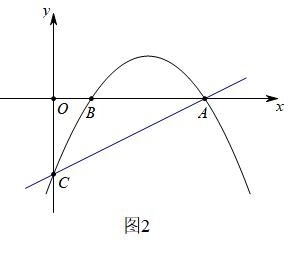
\includegraphics[scale=0.8]{figure/mj-14.png}
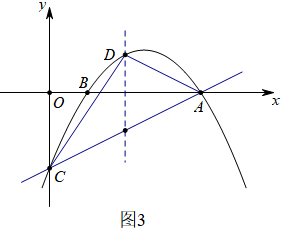
\includegraphics[scale=0.8]{figure/mj-15.png}
\end{minipage}

\end{document}